%Needs Package: 
%\usepackage{bm}
%\usepackage{multicol}
\section{LTI-Systeme}
\begin{multicols}{2}
    \subsection*{Linearität und Zeitinvarianz}
    \begin{itemize}
        \item $\mathcal{T}[x_1(t) + x_2(t)] = y_1(t) + y_2(t)$
        \item $\mathcal{T}[k_a \cdot x(t)] = k_a \cdot y(t)$
        \item $\mathcal{T}[x(t-t_0) = y(t-t_0)]$
    \end{itemize}

    \subsection{Beschreibung von LTI Systemen}

    \subsubsection{Impulsantwort}
    Impulsfunktion $\delta(t)$ wird am Eingang des Systems angelegt,
    die Reaktion darauf am Ausgang nennt man die \textbf{Impulsantwort} \bm{$h(t)$}.
    Sie beschreibt ein LTI-System vollständig.

    $$ y(t) = \mathcal{T}[x(t)]
        = \int \limits _{-\infty} ^{\infty} x(\tau) \cdot h(t-\tau)d\tau
        = x(t) * h(t)$$

    \subsubsection{Frequenzantwort}
    Die \textbf{Frequenzantwort} $\bm{H(\omega)}$ ist die Fouriertransformierte Impulsantwort.
    Sie ist eine komplexwertige dimensionslose Gewichstsfunktion.
    Auch sie beschreibt ein LTI-System vollständig.

    $$ Y(\omega) = X(\omega) \cdot H(\omega)$$

    \subsubsection{Berechnung des Ausgangssignals}
    1. Fourier-Transformation:  $X(\omega) = \mathcal{F}[x(t)]$ \\
    2. Berechnung in Frequenz:  $Y(\omega) = X(\omega) \cdot H(\omega)$ \\
    3. Rücktransformation:  $y(t) = \mathcal{F}^{-1}[Y(\omega)]$



    \subsection{Bezeichnungen}
    Übertragungsfunktion: $H(\omega)=|H(\omega)| \cdot e^{j\varphi_H(\omega)}$ \\
    Amplitudengang: $|H(\omega)|$ \\
    Phasengang: $\varphi_H(\omega)$ \\

    \subsubsection{Filtereigenschaften}
    $Y(\omega) = X(\omega) \cdot H(\omega)$ \\
    $|Y(\omega)| = |X(\omega)| \cdot |H(\omega)|$ \\
    $\varphi_y(\omega) = \varphi_x(\omega) + \varphi_H(\varphi)$

    \subsection{BIBO-Stabilität \tiny {Bound-Input-Bound-Output}}

    Systemantwort Begrenzt, wenn Eingangssignal Begrenzt
    \newline $\Rightarrow$ Konvergenzhalbebene Übertragungsfunktion enthält Imaginär-Achse
    \newline $\Rightarrow$ Alle Polstellen Übertragungsfunktion links von "$j$-Achse"
    \begin{center}
        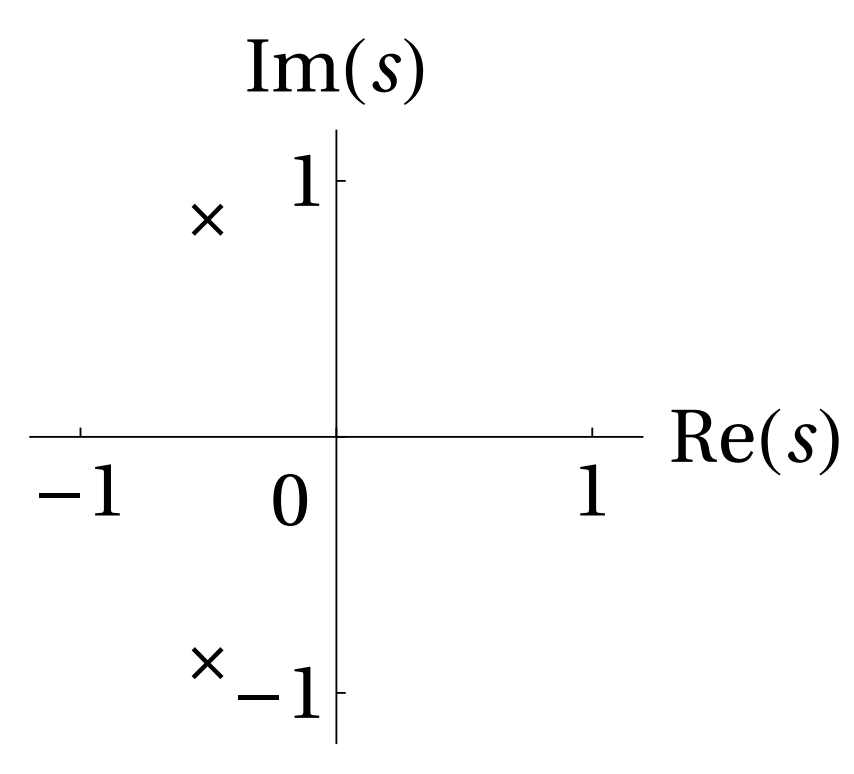
\includegraphics[width = 4cm]{include/Integraltransformationen/img/BiBo.png}
    \end{center}
\end{multicols}
